\documentclass[12pt,a4paper,ngerman]{article}
\usepackage{listings}
\usepackage{color}

\definecolor{dkgreen}{rgb}{0,0.6,0}
\definecolor{gray}{rgb}{0.5,0.5,0.5}
\definecolor{mauve}{rgb}{0.58,0,0.82}

\lstset{%
  language=Python,
  aboveskip=3mm,
  belowskip=3mm,
  showstringspaces=false,
  columns=flexible,
  basicstyle={\small\ttfamily},
  numbers=none,
  numberstyle=\tiny\color{gray},
  keywordstyle=\color{blue},
  commentstyle=\color{dkgreen},
  stringstyle=\color{mauve},
  breaklines=false,
  breakatwhitespace=true,
  tabsize=3
}
\usepackage[ngerman]{babel}
\usepackage[T1]{fontenc}
\usepackage{lscape}
\usepackage[utf8]{luainputenc}
\usepackage{relsize,etoolbox}
\usepackage[onehalfspacing]{setspace}
\usepackage{hyperref}
\usepackage{rotating}
\usepackage{xcolor}
\usepackage{xparse}
\usepackage[letterspace=900]{microtype}
\usepackage{lmodern}
\usepackage{fancyhdr}
\usepackage{graphicx}
\usepackage{float}
\usepackage{amsmath}
\usepackage{amsfonts}
\usepackage[hang,flushmargin]{footmisc}
\usepackage{tabularx}
\usepackage[font=smaller,labelfont=bf,skip=4pt,figureposition=top]{caption}
\captionsetup[figure]{position=above}
\usepackage{sectsty}
\usepackage{array}
\usepackage{tabu}
\usepackage{verbatim}
\usepackage{enumitem}

\usepackage[
  headheight=15pt,
  bmargin=34mm,
]{geometry}

\usepackage[
    % citestyle=authortitle-comp,  % this is too verbose!
    citestyle=authoryear-comp,
    bibstyle=numeric,
    % hyperref=false  % has to be set to false if you want to activate the hack which skips the "o.D." date
]{biblatex}

% Supress "n.d." (no date) entry for online references.
% \DeclareLabeldate[online]{%
%   \field{date}
%   \field{year}
%   \field{eventdate}
%   \field{origdate}
%   \field{urldate}
% }


% % Supress "n.d." (no date) entry for online references.
% % Use author instead of title for online cite
% %   https://stackoverflow.com/questions/69582838/biblatex-website-citation-is-italicized-and-uses-title-instead-of-author-when-r 
% \DefineBibliographyStrings{english}{nodate = {\ifboolexpr{test{\ifentrytype{online}}}{\hskip-.2777em}{n\adddot d\adddot}}}
% \DefineBibliographyStrings{german}{nodate = {\ifboolexpr{test{\ifentrytype{online}}}{\hskip-.2777em}{n\adddot d\adddot}}}



\newrobustcmd*{\parentexttrack}[1]{%
  \begingroup
  \blx@blxinit
  \blx@setsfcodes
  \blx@bibopenparen#1\blx@bibcloseparen
  \endgroup}

\AtEveryCite{%
  \let\parentext=\parentexttrack%
  \let\bibopenparen=\bibopenbracket%
  \let\bibcloseparen=\bibclosebracket}


\usepackage{tablefootnote}

% SET FONT
% \usepackage[cmintegrals,cmbraces]{newtxmath}\usepackage{ebgaramond-maths}\usepackage{helvet}
% \usepackage[cmintegrals,cmbraces]{newtxmath}
% \usepackage[T1]{fontenc}

\usepackage{fontspec}
\usepackage{ebgaramond}
\usepackage{ebgaramond-maths}

% \setmainfont{TeX Gyre Pagella}%% The Palatino from the TeX Gyre Project

% \makesavenoteenv{tabular}
% \makesavenoteenv{table}
\addbibresource{referencesbib.bib}

\sectionfont{\fontsize{14}{15}\selectfont}
\subsectionfont{\fontsize{12}{15}\selectfont}


\setlength\parindent{0pt}
\parskip2mm


% header and footer style
\pagestyle{fancy}
\fancyhead[R]{\slshape}
\fancyhead[L]{\slshape\nouppercase{\rightmark}}
\fancyfoot[C]{\thepage}
\renewcommand{\sectionmark}[1]{\markright{\thesection\ #1}}


% for tables side by side
% https://stackoverflow.com/questions/28678824/in-latex-how-to-put-two-separate-tables-side-by-side-on-top-of-the-paper
\def \hfillx {\hspace*{-\textwidth} \hfill}

% custom commands
\newcommand{\mailto}[1]{\href{mailto:#1}{#1}}

% Titel and author
% \title{
\includegraphics[width=0.8\textwidth]{pictures/folk_logoicemCMYKDT}\\
% Bewegte Stille: \emph{Euler Lattice Spirals Scenery}}
% 
% \author{Levin Eric Zimmermann\\
% {\normalsize \mailto{levin-eric.zimmermann@folkwang-uni.de}}}
% \date{20. September 2020}

\linespread{1.4}
\AtBeginEnvironment{quotation}{\smaller}
\AtBeginEnvironment{quote}{\smaller}

\begin{document}


%************************************TITLE PAGE**************************************%

\begin{titlepage}

\newcommand{\HRule}{\rule{\linewidth}{0.5mm}} % Defines a new command for the horizontal lines, change thickness here

\center% Center everything on the page
 
%----------------------------------------------------------------------------------------
%	HEADING SECTIONS
%----------------------------------------------------------------------------------------

% \textsc{\LARGE Folkwang Universität der Künste}\\[0.5cm] % Name of your university/college
% \textsc{\large Institut für Computermusik und Elektronische Medien}\\[0.5cm] % Minor heading such as course title

\includegraphics[width=0.8\textwidth]{pictures/folk_logoicemCMYKDT}\\[1cm] % Include a department/university logo - this will require the graphicx package
\textsc{\Large Bachelorprojekt Integrative Komposition}\\[0.5cm] % Major heading such as course name
% \textsc{\large Course code}\\[0.5cm] % Minor heading such as course title

%----------------------------------------------------------------------------------------
%	TITLE SECTION
%----------------------------------------------------------------------------------------

\HRule\\[0.4cm]
{\huge mutwo: eine Ereignis zentrierte Umgebung zur Formalisierung zeitbasierter Künste}\\[0.2cm]
\HRule\\[1.5cm]
 
%----------------------------------------------------------------------------------------
%	AUTHOR SECTION
%----------------------------------------------------------------------------------------

\noindent
\begin{minipage}[b]{.25\textwidth}
\end{minipage}%
\begin{minipage}[b]{.25\textwidth}
\begin{flushleft}
\textsc{Autor:}

\textsc{Email:}

\textsc{Matrikelnummer:}

\textsc{Betreuung:}
\end{flushleft}
\end{minipage}%
\begin{minipage}[b]{.5\textwidth}
\begin{flushleft}
Levin Eric Zimmermann % Your name

{\normalsize \mailto{levin-eric.zimmermann@folkwang-uni.de}}

2332991

Prof. Dr. Michael Edwards
\end{flushleft}
\end{minipage}

\vspace{2cm}


%----------------------------------------------------------------------------------------
%	DATE SECTION
%----------------------------------------------------------------------------------------

{\large 01. August 2022}\\[2cm] % Date, change the \today to a set date if you want to be precise

\vfill % Fill the rest of the page with whitespace

\end{titlepage}

% \maketitle
% \thispagestyle{empty}
\newpage


\tableofcontents


\newpage

%%%%%%%%%%%%%%%%%%%%%%%%%%%%%%%%%%%%%%%%%%%%%%%%%%%%%%%%%%%%%%%%%%%%%%%%%%%%%%%%%%%%%%%%%%%%
%%%%%%%%%%%%%%%%%%%%%%%%%%%%%%%%%%%%%%%%%%%%%%%%%%%%%%%%%%%%%%%%%%%%%%%%%%%%%%%%%%%%%%%%%%%%

\section{Einleitung}

\subsection{Komposition und Werkzeuge (I)}

\begin{quote}
    ``It would seem axiomatic that any music [\dots] reveals the philosophic attitude of its creator.
    It also seems self-evident that if his attitude is vigorous and individualistic, his practical requirements are not neccessarily satisfied by the traditions he was born to;
    they may even require direct antitheses.''~\parencite[S. 3]{genesisOfMusic}
\end{quote}

Komposition ist von einer unbestimmten Menge Werkzeuge bedingt.
Die Menge umfasst Kulturtechnologien wie Notation oder Stimmungen, Handwerk wie Instrumentenbau, Architekturen wie Konzerthäuser und \emph{pendapa}, soziale Strukturen des Musizierens oder mathematische und logische Denkmodelle.

Letztgenannte Teilmenge umfasst Stimmführungsregeln oder 12-Ton Reihen.
Sie können als eine Sequenz diskreter Handlungsschritte beschrieben werden, die Eingangswerte in Ausgangswerte transformieren (i.e. Algorithmen)~\parencite[S. 3]{introductionToAlgorithms}.
Algorithmische Komposition bezeichnet Komposition, die diese Werkzeuge verwendet~\parencite[S. 1]{algorithmicCompositionParadigms}.
% XXX: Satz kürzer machen, besser leserlich
% wie Stimmführungsregeln in Fugen oder 12-Ton Reihen.

Mit dem Aufkommen der Computer wurden traditionelle Werkzeuge digitalisiert.
Lejaren Hiller und Leonard Isaacson sind als erste Personen bekannt, die Algorithmen in einem Computersystem zum Zweck der Komposition implementierten~\parencite[S. 63]{algorithmicCompositionParadigms}.
Auf sie folgten weitere.
% Vielleicht Beispiele nennen? James Tenny, John Cage, etc.?
Mit fortschreitender Entwicklung wuchs die Notwendigkeit generische Programmbestandteile zu entwickeln, die in unterschiedlichsten Arbeiten wieder verwendet werden können (Bibliotheken oder Rahmen)~\parencite[S. 78]{paradigmsAndComputerMusic}.

Im Herbst 2020 kann ich eine Vielzahl von Softwarebibliotheken für algorithmische Komposition finden.
Unzufrieden mit bestehenden Lösungen beginnen Tim Pauli und ich eine autonome Lösung zu entwickeln.
Fast zwei Jahre später, im Sommer 2022, umfasst das resultierende \emph{mutwo} Ökosystem über 22000 Zeilen Quellcode und 430 Tests.
Seit initialer Entwicklung sind mithilfe des Projektes sechs Kompositionen entstanden.

In vorliegender Arbeit möchte ich \emph{mutwo} dokumentieren.
Quelloffen und mit der GPL-3.0 Lizenz veröffentlicht ist \emph{mutwo} für Dritte zugänglich.
Wirkliche Zugänglichkeit ist aber nur mit ausreichender Dokumentation gewährleistet.
Meine kompositorische Arbeit ist durch die Bemühungen unzähliger Menschen möglich, die Freie Software veröffentlichen~\footnote{Hier ist \emph{Frei} im Sinne der Definition der \emph{Free Software Foundation} (FSF) verstanden. Die FSF bezeichnet eine Software als Freie Software, falls sie von Benutzer:innen geteilt, gelesen und verändert werden darf~\parencite{freeSoftwareDefinition}.}.
Mit der Dokumentation \emph{mutwos} möchte ich einen Teil in die Gemeinschaften Freier Software zurückgeben.

\subsection{Komposition und Werkzeuge (II)}

% Absatz: Begründung Aufwand eigenes Werkzeug entwickeln
Was Partch mit ``praktische Notwendigkeiten'' bezeichnet, begreife ich als kompositorische Werkzeuge.
Das Zitat impliziert, dass diese mitnichten neutral sind, sondern sich in einem engen Austausch mit den inneren Vorstellungen der Werkschaffenden befinden.
Mit der autonomen Entwicklung akustischer Instrumente war es Partch möglich implizite Vorbedingungen der Komposition via expliziter Entscheidungen neu zu verhandeln.
% xxx: das koennte man schreiben, wenn man betonen will, warum es so sinn macht sich so sehr mit
% xxx: den grundsaetzlichen kompositionswerkzeugen zu beschaeftigen:
% xxx: Wahrscheinlich zu viel unwichtiges. Auserdem habe ich keine lust quellen zu suchen :)
% Der Fokus auf statische, periphere oder undifferenzierten Aspekte einer Tradition, mag verbindender Aspekt der Musik des 20. Jahrhunderts sein.
% Anton Webern, Luigi Nono oder John Cage befreiten Stille von seiner rhetorisch-devoten Funktion.
% Mit Helmut Lachenmann wurden undifferenzierte Nebengeräusche akustischer Instrumente zum präzise gestalteten Hauptschauplatz.
Die Begründung der Anstrengung für die kompositorische Praxis Programme zu entwickeln, deckt sich für mich mit seiner Begründung für die Konstruktion eigener Instrumente.
Vernachlässigte Eigenschaften in bestehender Software verhindern eine Kongruenz von innerer Vorstellung und praktischen Möglichkeiten.
Besonders die Voreingenommenheit populärer Musiksoftware ist bekannt.
% TODO(One more quote!)
% TODO(Add references!)
Andrew Gerzso benennt die von konventioneller Musik geprägten Annahmen eines Sequenzers~\parencite[S. 78]{paradigmsAndComputerMusic}.
Kyam Allami bemängelt die oberflächliche, exotisierende Repräsentationen außereuropäischer Tonsystemen in kommerzieller Musiksoftware~\parencite[S. 59f]{microtonalityAndTheStruggle}.
Aber auch esoterischere Technologien wie Softwarebibliotheken für algorithmische Komposition unterliegen inhärenten Limitierungen.

% Absatz: die Limitierungen in bestehender Software ist und was du anders machen wolltest (Motivation)
Limitierende Paradigmen mir bekannter Bibliotheken waren und sind ausschlaggebend für die Entwicklung \emph{mutwos}.
% eigentlich wie bei partch hat mich anfang die tonhöhen problematik gestört.
Meine initiale Begegnung mit Einschränkungen betraf Tonhöhenstrukturen.
In meiner kompositorischen Arbeit begreife ich Intervalle als ganzzahlige Frequenzverhältnisse (reine Stimmung).
Meine bevorzugte Tonhöhenrepräsentation von Verhältnissen befindet sich jenseits europäischer Tonhöhennamen oder der MIDI Spezifikation.

In der Bibliothek \emph{SCAMP} werden Tonhöhen als Gleitkommazahl repräsentiert, die für Tonhöhennummern der MIDI Spezifikation stehen~\parencite{scampNoteLikeDefinition}.
Die Software \emph{Euterpea} deklariert Tonhöhen als zweielementige Tupel.
Das erste Element ist ein Tonklassenname europäischer Tradition (zB. \texttt{cs} oder \texttt{fbb}) und das zweite eine natürliche Zahl zur Indikation der Oktave~\parencite{euterpeaPitchDefinition}.
Die Notenklasse der Bibliothek \emph{jMusic} definiert drei unterschiedliche Konstruktoren, um Tonhöhen festzulegen:
wird dem Tonhöhenargument natürliche Zahlen zugewiesen, werden diese als Tonhöhennummern der MIDI Spezifikation interpretiert.
Gleitkommazahl werden als Frequenz gelesen, Zeichenketten als europäische Tonhöhennamen.
Die innere Repräsentation der Klasse erlaubt nur die Darstellung in Frequenz oder MIDI Nummer, sodass Tonhöhennamen umgewandelt werden~\parencite{jMusicSource}.
In \emph{slippery-chicken} sind Tonhöhen über eine eigene Klasse implementiert.
Die Funktion \texttt{make-pitch} erzeugt eine neue \texttt{pitch}--Instanz.
Ähnlich wie bei \emph{jMusic} gibt es unterschiedliche mögliche Datentypen des notwendigen Arguments \texttt{pitch} der \texttt{make-pitch} Funktion.
Falls \texttt{pitch} ein Symbol oder eine Zeichenkette ist, wird das Argument als Tonname europäischer Tradition gelesen.
Ist \texttt{pitch} eine Zahl wird diese als die Frequenz der Tonhöhe interpretiert.
Der Klasse \texttt{pitch} sind Attribute zugewiesen wie zB. \texttt{midi-note}, \texttt{white-note}, \texttt{accidental} oder \texttt{frequency}~\parencite{slipperyChickenSource}.

% Mutwo grundsaetzliche Idee: Utopie, dass alle unterschiedliche Denkpositionen ermoeglicht werden (theoretisch)
% Aufbau Bachelor-Arbeit:
%   - kurzer Ueberblick bestehender Loesungen (sehr kurz, nicht fuer jede Software eigenes Kapitel, sondern nur kurzer Abschnitt pro Software und Zusammenfassung)
%   - Motivation & Absicht
%   - grundsaetliche abstrakte Spezifikation des Aufbaus der Software
%   - Programmierstragien zur Realisierung beschriebener Absicht
%   - Beispiel-orientierte Einfuehrung
%   - Fallstudien
%   - Conclusio

% \emph{Mutwo} ist von einer eigenen Vielzahl von Einschränkungen betroffen.


% Abstatz: Struktur BA Arbeit

% Code:
%   core: 4314
%   music: 8061
%   midi: 1528
%   csound: 385
%   abjad: 4017
%   reaper: 108
%   common: 1091
%   ekmelily: 1356
%   isis: 388
%   mbrola: 162
%   zimmermann: 335
%   mmml: 965
%
%   ==============
%     22710 lines


% Tests:
%   core: 146
%   music: 168
%   common: 16
%   midi: 41
%   abjad: 22
%   ekmelily: 9
%   csound: 8
%   isis: 4
%   mbrola: 7
%   reaper: 2
%   zimmermann: 8
%
%   =============
%     431 tests

%%%%%%%%%%%%%%%%%%%%%%%%%%%%%%%%%%%%%%%%%%%%%%%%%%%%%%%%%%%%%%%%%%%%%%%%%%%%%%%%%%%%%%%%%%%%
%%%%%%%%%%%%%%%%%%%%%%%%%%%%%%%%%%%%%%%%%%%%%%%%%%%%%%%%%%%%%%%%%%%%%%%%%%%%%%%%%%%%%%%%%%%%

\section{Umgebungen computergestützter Komposition}

% name
% veröffentlichungsjahr
% entwickler/institution
% lizenz
% kosten (2022)
% unterstützte Plattformen 
% Sprache (implementierung) 
% Sprache (Anwendung) 
% beschreibung
% aktiv
% notation
% midi
% gui
% 
% kulitta


\begin{landscape}
    \begin{table}[h!]

        \begin{center}

            \begin{smaller}

                \begin{tabularx}{22cm}{X X X X X X X X X}
                    \hline
                    Name &
                    Initiale Entwicklung &
                    Lizenz &
                    Kosten (2022) &
                    Kompatible Plattformen &
                    Implementiert in\dots &
                    Angewendet mit\dots & 
                    Westliche Notation &
                    MIDI \\ [0.5ex] 

                    \hline\hline

                    Common Music &
                    1989 &
                    Vizsage Public License &
                    -- &
                    Linux/GNU, macOS, Windows &
                    Common Lisp &
                    Common Lisp & 
                    ja &
                    ja \\[1cm]


                    JMusic &
                    1998 &
                    PSF License v2 &
                    -- &
                    Linux/GNU, macOS, Windows &
                    Java &
                    Java & 
                    ja &
                    ja \\[1cm]

                    OpenMusic &
                    1998 &
                    GPL v3.0 &
                    -- &
                    Linux/GNU, macOS, Windows &
                    Common Lisp &
                    OpenMusic & 
                    ja &
                    ja \\[1cm]

                    slippery-chicken &
                    2000 &
                    GPL v3.0 &
                    -- &
                    Linux/GNU, macOS, Windows &
                    Common Lisp &
                    Common Lisp & 
                    ja &
                    ja \\[1cm]

                    Abjad &
                    2013 &
                    GPL v3.0 &
                    -- &
                    Linux/GNU, macOS, Windows &
                    Python &
                    Python & 
                    ja &
                    nein \\[1cm]

                    Opusmodus &
                    2014 &
                    Properetär &
                    250€ - 399€ &
                    macOS &
                    Common Lisp &
                    Common Lisp & 
                    ja &
                    ja \\[1cm]

                    JythonMusic &
                    2014 &
                    GPL v2.0 &
                    -- &
                    Linux/GNU, macOS, Windows &
                    Jython &
                    Jython & 
                    ja &
                    ja \\[1cm]

                    Euterpea 2.0 &
                    2015 &
                    zlib &
                    -- &
                    Linux/GNU, macOS, Windows &
                    Haskell &
                    Haskell & 
                    ja &
                    ja \\[1cm]

                    SCAMP &
                    2019 &
                    GPL v3.0 &
                    -- &
                    Linux/GNU, macOS, Windows &
                    Python &
                    Python & 
                    ja &
                    ja \\%
                    [0.5ex]
                    \hline
                \end{tabularx}

            \end{smaller}

        \end{center}

    \caption{Liste aktiver Bibliotheken}
    \end{table}
\end{landscape}

\subsection{isobar}

\subsection{Abjad}

\subsection{SCAMP}

\subsection{Open Music}

\subsection{Opusmodus}

\subsection{Slippery Chicken}

\subsection{Strasheela}



%%%%%%%%%%%%%%%%%%%%%%%%%%%%%%%%%%%%%%%%%%%%%%%%%%%%%%%%%%%%%%%%%%%%%%%%%%%%%%%%%%%%%%%%%%%%
%%%%%%%%%%%%%%%%%%%%%%%%%%%%%%%%%%%%%%%%%%%%%%%%%%%%%%%%%%%%%%%%%%%%%%%%%%%%%%%%%%%%%%%%%%%%

\section{mutwo}

\subsection{Motivation}

% unzufriedenheit bestehender loesungen:
%   - schwierigkeit am rande von common-western-music etwas zu machen
%       - stimmungen
%       - aber auch andere notation: kepathian
%   - bei bestehenden loesungen: zu viel konzentration auf notation oder westliche musik

% wuensche von software:
%   - moeglichst wenig einschraenkungen (auch keine von denen ich heute denke dass sie ok sind)
%       - keine bestimmte aesthetik (ala slippery chicken)
%       - keine bestimmte arbeitsweise (ala scamp)
%       - medien-neutral
%       - protokoll-neutral
%       - software-neutral
%       - quelloffen und unabhaengig von (grossen) institutionen oder unternehmen
%       - möglichst offen verständlich
%       - hackable & configurable: wenige verstecke variablen
%   - erstmal als programmier-bibliothek gedacht und weniger als gui software
%   - OS (plattform) unabhängig

% einerseits möglichst flexibel
% andererseits möglichst leicht verständlich

% nicht per se widersprüchlich: denn es sollte einfach möglichst gut anpassbar sein für
% die eigenen zwecke, und das benötigt nunmalls flexibilität und aber auch verständlichkeit


\subsection{Softwarearchitektur}

\subsubsection{Komponenten und Beziehungen}

\subsubsection{Ereignisse}

Ein Ereignis beschreibt eine Bewegung in einem Koordinatensystem mit $n\in\mathbb{N}:n>0$ Dimensionen.
Die Bewegung wird durch $n$ Vektoren dargestellt.
Dimensionen können Zeit, räumlichen Achsen (X, Y und Z) oder theoretischen Konstrukte (zB. den Primzahlexponenten eines Tonnetzes) entsprechen.
% Wahrscheinlich unwichtiges Detail
% \footnote{%
%         In Version 0.61.0 von mutwos Kernpaket sind Ereignissen immer nur der Vektor \emph{Dauer} in der Dimension \emph{Zeit} zugeordnet.
%         Das ist ein Implementierungsdetail, was in zukünftigen Versionen anders umgesetzt werden mag.
% }

Ereignissen sind zusätzliche Objekte zugeordnet, die Eigenschaften der Bewegung definieren.
Ein zugewiesenes Objekt könnte für einen Klang zB. eine Tonhöhe sein.
Für eine zweidimensionale räumliche Bewegung wäre eine Farbe denkbar, für eine dreidimensionale Bewegung eine bestimmte Gangart.

In mutwos Terminologie werden Objekte, die als Attribute einem bestimmten Ereignis zugewiesen sind, als Parameter bezeichnet.
Weil auch Vektoren als Attribute einem Ereignis zugeordnet sind, sind sie nur eine besondere Unterkategorie von Parametern.
In mutwos objektorientiertem Paradigma sind Ereignisse und Parameter Klassen und deren Instanzen.

% Ich bin mir nicht sicher, ob diese Grafik so besonders informativ ist.

% \begin{figure}[h!]
%     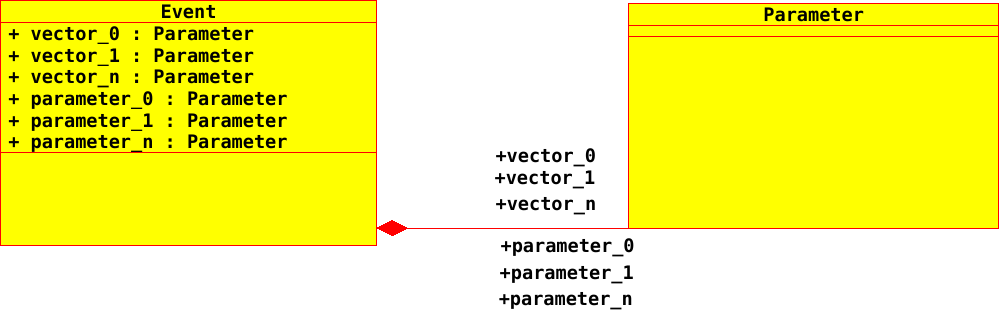
\includegraphics[scale=0.4]{uml_diagrams/event_parameter_basic_150.png}
% 
%     \caption{%
%         Ein Ereignis kann einen oder mehrere Vektoren enthalten.
%         Ein Ereignis kann einen oder mehrere Parameter enthalten.
%     }
% \end{figure}

\begin{table}[h!]
    \begin{center}
        \begin{tabular}{l l l l} 
            \hline
            Klassenname & enthält Ereignisse & innere Verhältnisse & Beispiel \\ [0.5ex] 
            \hline\hline
            \texttt{SimpleEvent} & nein & - & ein Ton, ein Strich \\ 
            \texttt{SequentialEvent} & ja & akkumulierend & eine Melodie, ein Quadrat \\ 
            \texttt{SimultaneousEvent} & ja & parallel & polyphoner Satz, zwei Rechtecke \\ [1ex] 
            \hline
        \end{tabular}
    \end{center}

    \caption{Kernereignisse in mutwo}
\end{table}

Ereignisse können andere Ereignisse enthalten oder keine anderen Ereignisse enthalten.
Falls Ereignisse andere Ereignisse enthalten, können die enthaltenen Ereignisse wiederrum iterativ weitere Ereignisse enthalten (Verschachtlung).
Falls ein Ereignis Ereignisse enthält, können diese entweder simultan oder sequenziell angeordnet sein.
Mit den drei Ereignisklassen \texttt{SimpleEvent}, \texttt{SequentialEvent} und \texttt{SimultaneousEvent} sind alle Möglichkeiten darstellbar.

\begin{figure}[h!]
    \begin{center}
        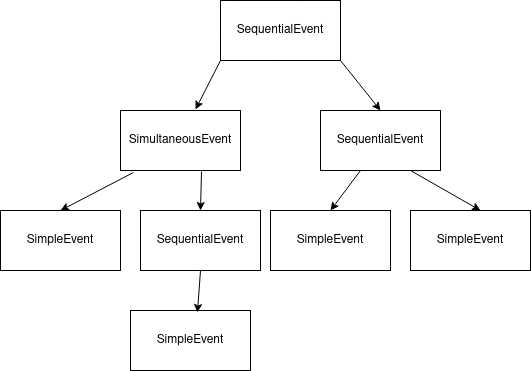
\includegraphics[scale=0.5]{pictures/nested_event.png}

        \caption{Exemplarische Verschachtlung von Ereignissen}
    \end{center}
\end{figure}


\subsubsection{Parameter}

Parameter repräsentieren generische Kategorien, die Ereignissen zugeordnet werden.
Generische Kategorien können beispielweise eine Farbe, eine Tonhöhe oder ein Luftdruck sein.

In mutwos Design sind Parameter als abstrakte Klassen definiert, die eine minimale, öffentliche Programmierschnittstelle beschreiben.
Diese minimale Schnittstelle versucht Parameter auf eine kompakte Identität zu reduzieren, die unabhängig ist von bestimmten Traditionen.
Wenn möglich besteht diese kompakte Identität aus nur einem Wert (zB. Zeichenkette oder Zahl).
Wenn möglich ist der Wert implizit einer physikalischen Einheit zugeordnet.

\begin{table}[h!]
    \begin{center}
        \begin{tabular}{l l l l} 
            \hline
            Parameter & Klassenname & Elementares Klassenattribut & Einheit \\ [0.5ex] 
            \hline\hline
            Tonhöhe & \texttt{Pitch} & \texttt{frequency} & Hertz \\ 
            Tonhöhenintervall & \texttt{PitchInterval} & \texttt{interval} & Cents \\ 
            Dauer & \texttt{Duration} & \texttt{duration} & beats \\ 
            Text & \texttt{Lyric} & \texttt{phonetic\_script} & X-SAMPA\footnotemark \\ 
            Lautstärke & \texttt{Volume} & \texttt{amplitude} & Volt \\ [1ex] 
            \hline
        \end{tabular}
    \end{center}

    \caption{Liste exemplarischer Ein-Wert-Parameter}
\end{table}

\footnotetext{%
    Das ``Extended Speech Assessment Methods Phonetic Alphabet'' ermöglicht die Darstellung der phonetischen IPA Symbole in ASCII.~\parencite{xsampaWikipedia}
}

Andere Bestandteile mutwos erwarten nur die minimal--definierte Schnittstelle.
Das ermöglicht Benutzern die Implementierung einer Repräsentation einer Kategorie, die der jeweiligen Interpretation entspricht.
Das Design mutwos versichert, dass die von Benutzern hinzugefügten Repräsentationen mit anderen Bibliothekskomponenten kompatibel sind.

\begin{figure}[h!]
    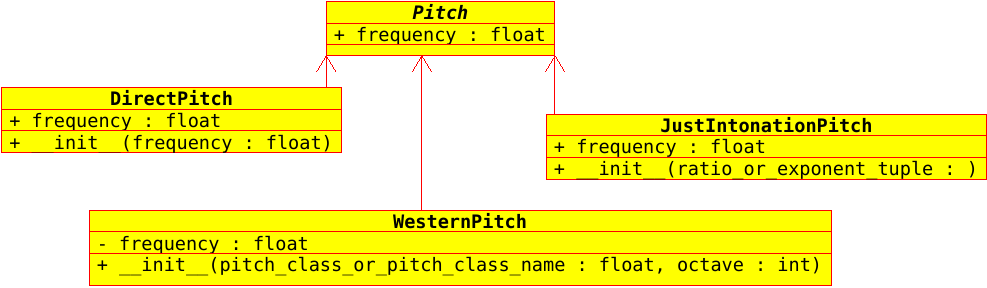
\includegraphics[scale=0.4]{uml_diagrams/pitches.png}

    \caption{%
        Schematische Darstellung eines Parameter und unterschiedlicher Subklassen.
        Die Subklassen werden mit unterschiedlichen Argumenten initialisiert.
    }

\end{figure}

\subsubsection{Übersetzer}

Ein Übersetzer transformiert eine Entität.
Entitäten sind entweder Objekte in Python oder externe Dateien.\footnote{%
    Objekte in Python können Instanzen von mutwo internen Klassen, dritten Bibliotheken oder nativen Klassen sein.
    Externe Dateien umfassen beispielweise Mididateien oder Textdateien.
}
Transformieren bedeutet hier entweder eine Veränderung des Inhalts oder eine Veränderung des Formats.


\begin{table}[h!]
    \hspace{-0.5cm}
        \smaller
        \begin{tabular}{l l l l} 
            \hline
            Klassenname & Eingangsentität & Ausgangsentität & Typ \\ [0.5ex] 
            \hline\hline
            \texttt{EventToMidiFile} & Instanz einer Ereignisklasse & Standard Midi File (SMF) & Format \\ 
            \texttt{MidiFileToEvent} & Standard Midi File (SMF) & Instanz einer Ereignisklasse & Format \\ 
            \texttt{TwoPitchesToCommonHarmonicTuple} & Zwei Tonhöheninstanzen & Instanzen gemeinsamer Harmonischer & Inhalt \\ 
            \texttt{PitchToTabulaturaPitch} & Tonhöheninstanz & Tonhöheninstanz & Inhalt \\ [1ex] 
            \hline
        \end{tabular}

    \caption{Exemplarische Übersetzer}
\end{table}


Übersetzer in mutwo folgen einem funktionalem Paradigma, dh.\ ein Übersetzer verändert nicht die Eingangsentität, sondern erzeugt eine neue, unabhängige Entität.
Das vereinfacht das Übersetzen derselben Entität mit unterschiedlichen Übersetzer.

\subsubsection{Generatoren}

Generatoren liefern (zumeist generische) Daten, die für generative Kunst nützlich sein mögen.
Generatoren umfassen Funktionen, Klassen, Konstanten oder andere Objekte.
Die Rückgabewerte der Funktionen und Klassen sind häufig Python native Objekte, die von Benutzern kreativ angewendet werden können.

\begin{table}[h!]
    \begin{center}
        \begin{tabular}{l l} 
            \hline
            Objekt & Beschreibung \\ [0.5ex] 
            \hline\hline
            \texttt{reflected\_binary\_code} & Erzeugt variable Gray-Codes \\
            \texttt{TUNEABLE\_INTERVAL\_TUPLE} & intonierbare Intervalle nach Marc Sabat \\
            \texttt{ActivityLevel} & Zyklen der Werte 0 und 1 nach Michael Edwards \\ [1ex] 
            \hline
        \end{tabular}
    \end{center}

    \caption{Exemplarische Generatoren}
\end{table}

\subsubsection{Module und Packete}

Der Quellcode von mutwo ist nach rigiden Regeln strukturiert.
Die Struktur basiert auf Pythons System von verschachtelten Modulen, Importe und Paketen.
Absicht der rigiden Struktur ist eine einfache Verwendung für Benutzer und eine Vereinfachung der Entwicklung und Instandhaltung eines komplexen Softwareprojekts.

Der Paketname der Bibliothek ist mutwo.
Pakete können im Python-Ökosystem auf der Plattform \emph{pypi} verwaltet werden.
Mit dem standardisierten Pythonpaketmanager \emph{pip} können Pakete von \emph{pypi} installiert werden.

\lstset{language=bash}

\begin{lstlisting}
    pip3 install mutwo
\end{lstlisting}

Das Paket mutwo ist in unterschiedliche Module geteilt.
Die unterschiedlichen Module korrelieren mit den zuvor beschriebenen elementaren Bestandteile von mutwo.
Sie werden flankiert von zusätzlichen Hilfsmodulen.

\begin{table}[h!]
    \begin{center}
        \begin{tabular}{l l} 
            \hline
            Modulname & Modulbeschreibung \\ [0.5ex] 
            \hline\hline
            \texttt{configurations} & Globale modulübergreifende Konfigurationsvariablen \\
            \texttt{constants} & Globale modulübergreifende Konstanten \\
            \texttt{converters} & Importieren und Exportieren von Daten, Übersetzen interner Strukturen \\
            \texttt{events} & Definition verschiedener Ereignisklassen \\
            \texttt{generators} & Generierung von für künstlerische Arbeiten hilfreiche Daten \\
            \texttt{parameters} & Klassen, deren Instanzen Ereignisattributen zugeordnet werden \\
            \texttt{version} & Versionsdefinition des Moduls \\
            \texttt{utilities} & Hilfsmethoden, Errordefinition \\ [1ex] 
            \hline
        \end{tabular}\label{table:modulDefinition}
    \end{center}

    \caption{Moduldefinitionen}
\end{table}

Module oder Pakete können in Python auf unterschiedliche Weisen importiert werden.
Die folgende Zeile dokumentiert die in mutwo bevorzugte Weise:

\lstset{language=Python}

\begin{lstlisting}
    from mutwo import parameters
\end{lstlisting}

Mutwo Module enthalten direkt die verwendbaren Objekte (Klassen, Funktionen).
Sie können nur eine limitierte Anzahl bestimmter Submodule enthalten.
Weil die Regel für alle mutwo Module gilt ist sie einfach zu verstehen für neue Benutzer.
Sie korreliert mit der fünften Zeile des \emph{Zen of Python}:

\begin{quote}
    ``Flat is better than nested.''
\end{quote}

Folgende Tabelle beschreibt die möglichen Submodule eines Moduls:

\begin{table}[h!]
    \begin{center}
        \begin{tabular}{l l} 
            \hline
            Submodulname & Modulbeschreibung \\ [0.5ex] 
            \hline\hline
            \texttt{abc} & Abstrakte Klassen, Definition der gemeinsamen API \\
            \texttt{configurations} & Globale modifizierbare Variablen zur Modulkonfiguration \\
            \texttt{constants} & Globale Konstanten des Moduls \\
            \hline
        \end{tabular}
    \end{center}

    \caption{Submoduldefinitionen}
\end{table}

Die Strukturierung des Quellcodes in thematisch getrennte Module und Submodule ist aber unzureichend.
Weil die grundsätzliche Designprämisse von sehr generischen Strukturen ausgeht, die aber präzise spezifiziert werden können, ist der potenzielle Umfang der Bibliothek schwer fasslich.
In mutwo ist das Problem durch eine modulare Struktur von thematisch getrennten Paketen gelöst.
Jedes Paket hat einen eigenen Namen auf \emph{pypi}, hat eine eigene, unabhängige Version, kann eigene Abhängigkeiten definieren und ist je nach Abhängigkeitsstruktur unabhängig von anderen Paketen installierbar.

Die modulare Strukturierung in separate Pakete hilft nicht nur der Entwicklung und Instandhaltung, sondern ermöglicht auch Nutzern nur diejenigen Programmbestandteile zu installieren, die für ein bestimmtes Projekt benötigt werden.
Das macht die Bibliothek leichter.
Mit der modularen Struktur können Dritte unkompliziert die Bibliothek durch weitere Funktionen erweitern.
Sie können einfach ein neues Paket dem mutwo Ökosystem hinzufügen.

Technisch ist die Modularität durch Pythons Unterstützung von \emph{namespace packages} gelöst.
Das ermöglicht voneinander unabhängigen Pakete die Installation von Quellcode unter einem gemeinsamen Paketnamen.

Einzelne Pakete im mutwo Ökosystem sind auf standardisierte Weise benannt.
Ihr Name setzt sich durch das Wort \emph{mutwo} und einem Begriff für die enthaltenen Funktionen zusammen:

\begin{itemize}
    \item{\textbf{mutwo.core}: Kunstform-, medien- und kulturagnostische Objekte}
    \item{\textbf{mutwo.music}: Musikspezifische Objekte}
    \item{\textbf{mutwo.reaper}: Funktionen die mit der DAW Reaper zusammenhängen}
    \item{\dots}
\end{itemize}

Das mutwo Ökosystem setzt die anfänglich beschriebene Struktur von Modulen und Submodulen auch in separaten Paketen um.
Die Namen der Module sind allerdings Kompositionen aus einem Präfix und einem Suffix.
Der Präfix ist der Suffix des Paketnamen (zB. \texttt{core} oder \texttt{music}).
Der Suffix beschreibt die Funktion des Moduls (zB. \texttt{events} oder \texttt{parameters}, siehe Tabelle~\ref{table:modulDefinition}).
Präfix und Suffix sind durch einen Unterstrich getrennt:

\begin{itemize}
    \item{\texttt{core\_parameters}}
    \item{\texttt{music\_events}}
    \item{\texttt{midi\_converters}}
\end{itemize}

Das Importieren im Quellcode funktioniert auf gleiche Weise wie oben beschrieben:


\begin{lstlisting}
    from mutwo import core_parameters
    from mutwo import music_events
    from mutwo import midi_converters
\end{lstlisting}

%%%%%%%%%%%%%%%%%%%%%%%%%%%%%%%%%%%%%%%%%%%%%%%%%%%%%%%%%%%%%%%%%%%%%%%%%%%%%%%%%%%%%%%%%%%%
%%%%%%%%%%%%%%%%%%%%%%%%%%%%%%%%%%%%%%%%%%%%%%%%%%%%%%%%%%%%%%%%%%%%%%%%%%%%%%%%%%%%%%%%%%%%

\subsection{Strategien zur Umsetzung generischer, flexibler Strukturen}

\subsubsection{Abstrakte Klassen}

\subsubsection{Funktionen als Argumente}

\subsubsection{Dynamische Zuweisung von Attributen}

\subsubsection{Trennung von format-, programm-, protokollspezifischen Darstellungen und interner Repräsentation}

\subsubsection{Abwesenheit vorgegebener Arbeitsmodelle}

\subsubsection{Deskriptive Fehlermeldungen und Warnungen}

\subsubsection{Warnungen statt Fehler}

\subsubsection{Konfigurierbare globale Standardwerte (``convention over configuration'')}

%  \footnote{https://en.wikipedia.org/wiki/Convention\_over\_configuration}

\subsubsection{Annotation von Typen im Quellcode}

\subsubsection{Rigide Namenskonventionen}

\subsubsection{Dokumentation der API}

%%%%%%%%%%%%%%%%%%%%%%%%%%%%%%%%%%%%%%%%%%%%%%%%%%%%%%%%%%%%%%%%%%%%%%%%%%%%%%%%%%%%%%%%%%%%
%%%%%%%%%%%%%%%%%%%%%%%%%%%%%%%%%%%%%%%%%%%%%%%%%%%%%%%%%%%%%%%%%%%%%%%%%%%%%%%%%%%%%%%%%%%%

\subsection{Beispiel-orientierte Einführung}

%%%%%%%%%%%%%%%%%%%%%%%%%%%%%%%%%%%%%%%%%%%%%%%%%%%%%%%%%%%%%%%%%%%%%%%%%%%%%%%%%%%%%%%%%%%%
%%%%%%%%%%%%%%%%%%%%%%%%%%%%%%%%%%%%%%%%%%%%%%%%%%%%%%%%%%%%%%%%%%%%%%%%%%%%%%%%%%%%%%%%%%%%

\subsection{Fallstudien}

\subsubsection{thanatos trees for Tim Pauli}

\subsubsection{ohne Titel (2) und ohne Titel (3)}

\section{Zusammenfassung}

\subsection{Richtungen weiterer Entwicklungen}

\subsection{Evaluation}

\newpage

\appendix

\printbibliography

\newpage

\listoffigures

\newpage


\end{document}
